\documentclass[FM,BP]{tulthesis}  % Bakalářská práce fakulty mechatroniky
\usepackage[czech]{babel}  % Česká šablona dokumentu
\usepackage[utf8]{inputenc}  % Česká diakritika
\usepackage{graphicx}  % Tvorbě tabulek
\usepackage{float}  % Ukotvení věcí na svém místě (obrázky, tabulky, grafy, ...)
\usepackage{hyperref}  % Klikací odkazy v obsahu a referencích
\usepackage{gensymb}  % Pro stupne celsia
\usepackage{url}  % Pro lomeni adres url

\TULtitle{Koncept nízkonákladového sledovacího zařízení pro osobní automobily}{The concept of a low cost tracking device for personal cars}
\TULprogramme{B2646}{Informační technologie}{Information Technology}
\TULbranch{1802R007}{Informační technologie}{Information Technology}
\TULauthor{Tomáš Moravec}
\TULsupervisor{Ing. Lenka Kosková Třísková}
\TULyear{2016}

\begin{document}
\ThesisStart{male}

\begin{acknowledgement}
Děkuji vedoucí práce paní Ing. Lence Koskové Třískové za odborné vedení a poskytnuté informace při zpracování závěrečné bakalářské práce. Mé poděkování patří též Tomáši Stránskému za sdílení praktických zkušeností s použitými komponenty.
\end{acknowledgement}

\begin{abstractCZ}
Práce se zabývá problematikou sledovacích zařízení pro osobní automobily. V úvodu je definován pojem sledovacího zařízení a požadovaných vlastností. Následuje rešerše aktuální situace na trhu a srovnání užitých konceptů pro realizaci sledovacích zařízení. Na základě rešerše je navržen koncept sledovacího zařízení pro osobní automobily s cílem vytvořit levné a spolehlivé zařízení pro střední a nižší třídu vozů. Výstupem práce je prototyp cílového zařízení, který demonstruje zvolené hardwarové i softwarové řešení.
\end{abstractCZ}

\vspace{2cm}

\begin{abstractEN}
Thesis deals with tracking devices for cars. The introduction defines the concept of surveillance equipment and required attributes. Followed by a research of the current market situation and comparison of the concepts used for implementing surveillance equipment. Based on the research is designed concept of tracking devices for cars in order to create a cheap and reliable device for middle and lower class cars. The outcome of this work is the prototype of the target device, which demonstrates the chosen hardware and software solution.
\end{abstractEN}

\tableofcontents
\clearpage

\begin{abbrList}
\textbf{SMS} & Short message service, služba pro přenost krátkých textových zpráv\\
\textbf{GPS} & Global Positioning System, družicový polohovací systém\\
\textbf{GSM} & Groupe Spécial Mobile, globální systém pro mobilní komunikaci\\
\textbf{GPRS} & General Packet Radio Service, služba pro přenos dat v mobilní síti\\
\textbf{GLONASS} & Globalnaja navigacionnaja sputnikovaja sistěma, globální navigační satelitní systém\\
\textbf{IDE} & Integrated development environment, integrované vývojové prostředí\\
\textbf{LED} & Light-Emitting Diode, dioda emitující světlo\\
\textbf{ASCII} & American Standard Code for Information Interchange, americký standardní kód pro výměnu informací\\
\end{abbrList}

% Úvod

\chapter{Úvod}
Podnětem pro vytvoření této práce mi byl můj vlastní zájem o sledovací zařízení do vozidla, kdy jsem pátral po levném, kvalitním a jednoduše ovladatelném zařízení, jež naplní mé požadavky. Nejdříve jsem provedl průzkum českého trhu, kde jsem zjistil, že zařízení, která splňují mé požadavky, jsou cenově ohodnocena kolem 8 000 Kč, neboť všeobecně platí, že zařízení z dovozu jsou někdy i o polovinu levnější. Z tohoto důvodu jsem se rozhodl pro nákup z Číny. První zařízení za 500 Kč, které i přes oficiální informace o funkčnosti po celém světě, nebylo v České republice funkční, neboť mapové podklady na Evropu nebyly připraveny a odpovědi SMS chodily v čínském jazyce. Zároveň nebylo možné jej přepnout a i manuál byl pouze čínsky. Další pokus byl se zařízením za 1 000 Kč, kdy mapové podklady byly tentokrát přes mapy Google, a byly tedy funkční. Zařízení ale v SMS odpovídalo špatně srozumitelnými textovými řetězci, přesnost na stovky metrů byla nedostatečná a poloha byla tedy určena vždy o několik ulic vedle. Stále jsem hledal vhodné řešení dané situace, a proto jsem se rozhodl pro výrobu vlastního sledovacího zařízení, které by bylo možné pořídit v co nejnižší cenové hladině, ale s vlastnostmi náročnějších modelů, jež jsou v podstatně vyšší cenové relaci. Svým výzkumem jsem zjistil, že toto lze realizovat. K lepší motivaci k dokončení svého výzkumu, jsem se rozhodl, že v rámci své bakalářské práce provedu první etapu, tedy vytvoření funkčního prototypu a návrhu programové části.

% Sledovací zařízení

\chapter{Sledovací zařízení}
Sledovací zařízení je přístroj, udávající svou vlastní polohu na planetě Zemi, pomocí zeměpisné šířky a délky. Poloha se určuje vzhledem k systému družic GPS, které obíhají rovnoměrně rozprostřeny na oběžné dráze země. Typicky slouží ke sledování osob, vozidel, či nákladu a jeho využití najdou jak běžní domácí uživatelé a bezpečnostní agentury, usilující o bezpečnost vozidel, podniky monitorující pohyb svého vozového parku (Fleet management), tak i  velké logistické společnosti, sledující pohyby zásilek nebo kontejnerů. Přesnost polohy je pro uživatelský sektor desítky metrů, zatímco autorizovaní uživatelé (americká armáda a vybrané spojenecké armády) mají k dispozici přesnost v jednotkách metrů. Vyšší přesnosti se dosahuje způsoby, jako jsou například mobilní sítě, jiné navigační systémy, matematické výpočty atd. Za ideálních podmínek lze přesnost zvýšit i na jednotky centimetrů. Přesnost vertikální je zpravidla 2x až 3x tak horší než zmiňovaná horizontální \cite{gpsCommon}.

\section{Historie}
Polohovací systém GPS je vojenský globální družicový systém \cite{what}, provozovaný Ministerstvem obrany Spojených států amerických. Projekt navazuje na předchozí NAVSTAR GPS a od roku 1978 bylo do dnešního dne vypuštěno celkem 32 družic. Družice nebyly vypouštěny pouze za účelem určování polohy pro navádění raket a dalších zařízení, ale také aby detekovaly vypuštění balistických raket a výbuchy jaderných bomb. Všechny satelity byly také vybaveny přesnými atomovými hodinami, které dnes dodávají přesný čas po celé zemi. Původně vojenský projekt se stal dostupným i pro neautorizované uživatele z finančních důvodů, aby nemusel být zrušen. V roce 1990 během války v Zálivu byla dočasně deaktivována dostupnost pro neautorizované uživatele a zapojena byla opět v roce 1991  \cite{guide}.

\section{Přítomnost}
Satelitní systém GPS se stal synonymem pro sledovací zařízení a určování polohy a je celosvětově využíván ve všech lidských odvětvích. Nicméně dnes není jediným projektem poskytujícím zeměpisnou polohu. Od roku 2011 je k dispozici ruský armádní polohový systém GLONASS, který se vyznačuje stejnou přesností jako systém GPS \cite{glonass}. Pomalu, ale jistě se dostává do povědomí a většina nejnovějších mobilních zařízení umí komunikovat nejenom s GPS, ale také s GLONASS. Získáváním dat z více než jednoho systému satelitů, poskytuje výrazné zvýšení přesnosti polohy. Posledním, zatím nedokončeným, je evropský navigační systém Galileo, který má od roku 2012 nové sídlo v Praze. Částečně měl být funkční v roce 2015 (18 satelitů) a plně dokončen roku 2019/20 (30 satelitů). V roce 2014 však přišel systém o dvě nové družice, které měl vynést ruský nosič. Bohužel mu selhal poslední stupeň rakety a obě byly vyneseny na špatnou oběžnou dráhu, na které jsou dodnes. Později roku 2014 byla vypuštěna první družice na správnou oběžnou dráhu, ale přesto byl poté projekt pozastaven do doby, než se vyřeší, jak do systému zapojit družice na špatné oběžné dráze \cite{gps}.

% Požadované vlastnosti

\section{Požadované vlastnosti}
V honu za kvalitním, ale levným sledovacím zařízením, je nutné nalézt kompromis mezi nízkou cenou a pohodlím zákazníka. K zajištění tohoto cíle je třeba vyzdvihnout vlastnosti, které neovlivní cenu, ale výrazně posílí funkčnost a tím i konkurenceschopnost zařízení. Následující vlastnosti pro mne budou hrát důležitou roli při výběru hardwarových součástek, stejně tak mi pomohou se zaměřit na části kódu, které potřebují být optimalizovány nejlépe.

\subsection{Cena}
Koncept bude primárně zaměřen na minimalizaci případné výrobní ceny s ohledem na zachování všech funkcí, očekávaných od sledovacího zařízení. Aby byl produkt atraktivní, ale levný, je důležité kvalitní zpracování částí, které neovlivní konečnou cenu zařízení. Jedná se o programovou část, jež je slabým článkem většiny dostupných modelů, v kategorii nízkonákladových sledovacích zařízení. Dostupným modelem je v této práci myšleno sledovací zařízení, běžně dostupné v českých kamených, nebo internetových obchodech. Velkou úsporu peněz bude mít připojení na autobaterii, kde levné modely touto možností neoplývají a jsou cenově zatíženy drahými bateriemi, které jsou mnohdy tou nejdražší částí sledovacího zařízení. V závěrečné fázi se budu pokoušet odstranit přebytečné funkce, zbytečně komplikující provoz a přispívající k vyšší ceně.

\subsection{Spolehlivost}
Zařízení musí být spolehlivé a poskytovat požadované informace za jakýchkoliv podmínek a to i při nízké ceně vybavení. V případě poruchovosti u běžně dostupných modelů, když vynecháme faktory, které nelze ovlivnit, například nedostupný signál GPS nebo GSM sítě, je na vině buď ztráta signálu špatným umístěním ve vozidle (o správném umístění je nutné zákazníka informovat), vybití baterie, softwarová chyba která způsobí zacyklení, nebo při provádění různých operací ignoruje příchozí SMS. Proto je nutné číst a obsloužit všechny doručené SMS a informovat uživatele o všech skutečnostech, například o výpadku signálu, při žádosti o získání polohy.

\subsection{Bezpečnost}
Žádný z dostupných modelů, v kategorii nízkonákladových zařízení, nemá možnost nastavení řídících čísel, nebo hesla pro obnovení, při jeho ztrátě. Kdyby případný zloděj zjistil telefonní číslo, ať už odposlechem poblíž vozidla, nebo z telefonu majitele, je schopný deaktivovat zařízení na dálku a odcizit vozidlo bez sebemenšího podezření majitele. Proto je nutné myslet na bezpečnost jak při pokusu o vypnutí z cizího čísla, tak při případném odpojení od zdroje napájení, které by ve finální verzi jistila integrovaná baterie o malé kapacitě, a zajistila by pouze odeslání varovné SMS. Je pravděpodobné, že při odpojení od baterie by bylo sledovací zařízení odstraněno z vozidla a delší výdrž by byla zbytečná. Díky tomu se dá ušetřit na ceně, která je z velké části tvořena potřebou velkých baterií.

\subsection{Nenáročnost}
Zařízení musí být nenáročné na údržbu, to znamená například výměnu, nebo dobíjení baterií. Baterie by měla být v ideálním případě připojena k autobaterii, která dodává energii i když je motor vozidla vypnutý. Na druhou stranu, jeho spotřeba nesmí ovlivnit chod vozu, například vybitím autobaterie. Taková situace může při déle vypnutém motoru nastat velice snadno, protože spotřeba při připojení do sítě GPS je extrémně vysoká. Řešením by mělo být připojení pouze do telefonní sítě GSM, kde se bude čekat na příkazy z autorizovaného telefonního čísla. V případě neoprávněného pohybu vozidla, nelze sledovat pohyb vozu pomocí GPS, protože spotřeba by byla příliš vysoká. Je nutné najít alternativní řešení v podobě jednoho z dostupných senzorů. Běžně využívané jsou vibrační senzory, nebo senzor zrychlení, tedy akcelerometr. Ty zajistí připojení do sítě GPS, pouze v případě pohybu a tedy i minimalizují spotřebu.

\subsection{Vícejazyčnost}
Z hlediska českého trhu, je nevýhodou všech nízkonákladových a většiny sledovacích zařízení střední třídy, orientace na pouze jediný jazyk a to anglický. Jazyka neznalý uživatel může být zmatený a v nestandardních situacích odkázaný pouze na manuál, které některé modely ani nemají. Většina dostupných modelů je přeprodejem čínských zařízení a zřídkakdy jsou k nim dodávány manuály v anglickém jazyce. Je tedy věcí přeprodejce, zda vytvoří český manuál. Není to problém pouze České republiky a vzhledem k tomu, že se jedná o jednoduchou softwarovou implementaci, základní komunikační rozhraní bude v českém jazyce s možností jednoduchého přepnutí na požadovanou jazykovou lokalizaci. Do finálního produktu bude pouze stačit nahrát dostatečné množství jazykových variant, které vzhledem k nízkému počtu textových řetězců a nenáročnosti jejich uložení v paměti, nebude mít žádný vliv na případnou cenu, která by jinak mohla být způsobena nutností navýšení paměti pro data.

\subsection{Nastavitelnost}
Další z nevýhod dostupných produktů je nemožnost jakéhokoliv vlastního nastavení či personalizace. Ať už se jedná o citlivost senzorů, počet potřebných satelitů pro určení polohy (čím méně satelitů, tím menší přesnost, ale větší šance na získání polohy při špatném signálu), nebo nastavení jednotlivých textových řetězců. Vždy je dobré, aby měl zákazník možnost si své zařízení přizpůsobit dle libosti. Tuto možnost mu zařízení bude nabízet a vzhledem k tomu, že implementace je čistě softwarová záležitost, nebude tím ovlivněna finální cena.

\subsection{Přívětivost}
SMS s řídícími příkazy musí být jednoduché, uživatelsky přívětivé a snadno zapamatovatelné, aby bylo pro zákazníka ovládání intuitivní a srozumitelné. Nejpřívětivější a nejjednodušší je to, co je pro uživatele nejpřirozenější, tedy běžná slova a věty, stejně tak sledovací zařízení by ve stejné formě mělo i odpovídat. Tedy komunikace mezi uživatelem a sledovacím zařízením by měla být formou konverzace. Například \uv{Kde jsi?}, odpověď: \uv{Probíhá lokalizace, poloha bude zaslána během několika minut}, později: \uv{Nacházím se na souřadnicích xxx}. Stejně tak instalace zařízení musí být jednoduchá a nesmí jí provázet komplikované nastavování. Vše by mělo fungovat při prvním spuštění automaticky.

\section{Normy}
S pomocí vedoucí práce jsem prostudoval stávající normy, za účel připravenosti na případné reálné použití. Prvním byla Ergonomie softwaru pro multimediální uživatelská rozhraní - Část 2: Multimediální navigace a ovládání, jejíž obsah ale neodpovídá mé práci, dále pak obecné normy pro elektrická zařízení do vozidel a zákon o podmínkách provozu vozidel, který se zabývá zejména homologací. Jejich studií bylo zjištěno, že mé sledovací zařízení žádnou z norem neporušuje a tato tvrzení bylo ověřena i po dokončení práce. Prostudované normy jsou zmíněny níže.

\paragraph{Seznam zkoumaných norem:}
\begin{itemize}
\item ČSN EN ISO 14915-2 (833581)
\item ČSN 30 4002 (304002)
\item ČSN 30 4003 (304003)
\item ČSN ISO 6722-3 (304004)
\item ČSN 30 4011 (304011)
\item ČSN EN 1648-1 (304020)
\item ČSN EN 1648-2 (304020)
\end{itemize} 

% Situace na trhu

\chapter{Situace na trhu}
Na českém ani žádném sousedním trhu nejsou k dispozici evropské výrobky v kategorii nízkonákladových sledovacích zařízení, která by byla veřejně dostupná. Veškeré zboží je dováženo od čínských dodavatelů, takže žádný z přístrojů nemůže reflektovat požadavky evropských zákazníků. Domácí výrobky existují až od kategorie drahých sledovacích zařízení, které jsou však pro běžného zákazníka nedostupné, nebo jsou zatíženy měsíčními poplatky za využívání služeb od jejich poskytovatele. V následujícím textu rozdělím český trh na kategorie a následně se budu věnovat pouze dvěma nejlevnějším z nich, protože drahé a specializované systémy nejsou předmětem této práce.

\section{Kategorie}
Vzhledem k tomu, že se mi nepodařilo dohledat žádné dělení, roztřídím zařízení na trhu dle vlastních cenových hladin, pro které jsou společné specifické vlastnosti a funkce.

\subsection{Nízkonákladová zařízení (do 2 000 Kč)}
Kategorie těch nejlevnějších sledovacích zařízení se mnohdy neoznačují ani jako sledovací zařízení pro automobily. Většinou jsou určeny pro vhození do brašny, nošení na ruce, nebo přivěšení na klíčenku, kde se sesbíraná data o poloze ukládají na malou paměťovou kartu, ze které jsou později vyčteny do počítače. Jen zřídka mají zařízení v této kategorii možnost odesílání SMS přes síť GSM. Vždy mají integrovanou baterii, která při běžném používání vydrží v rámci jednotek dnů, poté je nutné zařízení dobít. Vyznačují se nemožností napojení na autobaterii nebo jakékoliv nastavení.

\paragraph{Specifické vlastnosti této kategorie:}
\begin{itemize}
\item baterie (výdrž jednotky dnů)
\item ukládání polohy na paměťovou kartu
\end{itemize}

\subsection{Střední třída (2 000 až 8 000 Kč)}
Střední třída je již plnohodnotnou kategorií sledovacích zařízení do automobilů, cena zařízení se ve většině případů pohybuje kolem 6 000 Kč, nicméně vlastnosti této kategorie se objevují ihned za hranicí 2 000 Kč. Nejlevnější z této kategorie mají většinou pouze notifikační SMS a baterii s výdrží několika dnů, ale ve většině případů dražších strojů, obsahují silnější baterii, která je schopna vydržet desítky dnů. Zároveň obsahují levné senzory pohybu, které bohužel nemají nastavitelnou přesnost a ve většině případů je zde možnost měsíčních poplatků za služby webové nebo mobilní aplikace, ve které je možné nejenom sledovat polohu vozu, ale také nastavit funkci takzvaně geofence, tedy kruhové oblasti kolem zvolené polohy, která když je překročena (například když vozidlo opustí město), zákazník je informován. V krajních případech mají možnost připojení na autobaterii a tedy uložení do motoru vozidla. V jiném případě mají silné magnety, umožňující přichycení, například na podvozku vozidla. Přes SMS příkazy lze nastavit autorizovaná telefonní čísla.

\paragraph{Specifické vlastnosti této kategorie:}
\begin{itemize}
\item baterie (výdrž desítky dnů)
\item SMS notifikace
\item možnost připojení na autobaterii
\item mobilní/webová aplikace pro sledování polohy za měsíční poplatek
\item možnost nastavení autorizovaných čísel
\item magnetické úchytky
\end{itemize}

\subsection{Profesionální řešení (8 000 až 20 000 Kč)}
Profesionální řešení jsou téměř vždy napojena na autobaterii a na sběrnici vozidla. Jejich dálkovým řízením pomocí webového rozhraní lze například sledovat přívod paliva, stav nádrže, dalších kapalin a efektivně mít pod kontrolou celou síť firemních vozidel, monitorovat a optimalizovat trasy. Jsou vybaveny silnými bateriemi a odolné proti poškození. Umožnují například připojení kamerových systémů, nebo připojení mikrofonu do kabiny řidiče pro případné urychlené jednání s pojišťovnou. Bohužel jeho provoz a instalace je finančně velice náročná a proto se vyplatí pouze pro společnosti s velkým vozovým parkem. Využití najde i na moři v lodní i kontejnerové dopravě. Tento typ řešení v České republice poskytuje například společnost Jablotron, nebo Škoda. Obě společnosti jsem kontaktoval, ale v rámci utajení výzkumu odmítly sdílet informace. Nepokoušel jsem se o jejich další zjištění, neboť profesionální zařízení nejsou cílem této práce. 

\paragraph{Specifické vlastnosti této kategorie:}
\begin{itemize}
\item bezdrátové řízení a monitoring
\item připojení na autobaterii
\item připojení na komunikační sběrnici vozu
\item baterie (výdrž desítky dnů)
\item připojení kamerových zařízení včetně mikrofonu
\item vyžaduje odbornou montáž a údržbu
\end{itemize}

\subsection{Specializovaná zařízení (od 20 000 Kč)}
Specializovaná sledovací zařízení jsou raritou, určenou především pro kategorie luxusních vozů třídy A. Dle telefonické konzultace u společnosti SHERLOG, se vyplatí montáž těchto zařízení až do vozidel s cenou převyšující 3 000 000 Kč. Zařízení jsou sofistikovaně ukryta na složitě dostupných místech, ve většiné případů jsou rozdělena na více částí po celém voze, aby nebylo jednoduché je vyřadit. Jsou jištěna proti odstranění a v případě krádeže vozu umožňují okamžité odpojení a převzetí specifických částí vozu, například plynulé zastavení vozidla. Monitoring probíhá neustále a bezpečnostní agentura má vždy připravené vlastní vozy, které zabezpečí vozidlo i zloděje. Tyto služby v České republice poskytuje například firma SHERLOG, která jako ostatní společnosti nezveřejňuje ceny, ani technické parametry. Nepokoušel jsem se o jejich zjištění, neboť specializovaná zařízení nejsou cílem této práce. 

\paragraph{Specifické vlastnosti této kategorie:}
\begin{itemize}
\item nepřetržité sledování
\item převzetí kontroly vozidla
\item zajištění vozu v případě krádeže
\item velice obtížné odpojení, nebo poškození jednotky
\end{itemize}

% Porování kategorií

\section{Tabulka vlastností kategorií}
Následující tabuka shrnuje všechny zjištěné vlastnosti do jedné ucelené tabulky, ze které jsou lépe patrné rozdíly mezi jednotlivými kategoriemi. Symbolem \uv{x} je označena vlastnost, která je pro kategorii standardní a prázdným políčkem, neobsahující symbol \uv{x}, označuje tu vlastnost, která není pro kategorii standardní. Standardní je myšlena ta vlastnost, kterou mají společnou všechna zařízení v dané kategorii, naopak nestandardní je myšlena ta vlastnost, kterou nemají všechny, nebo většina zařízeních v dané kategorii společnou.

\renewcommand{\arraystretch}{1.5}
\begin{table}[H]
\begin{center}
\begin{tabular}{| l | c | c| c | c |}
\hline
Vlastnost & Nízkonákladová & Střední & Profesionální & Specializovaná\\
\hline
\hline
Baterie & x & x & x & x\\
\hline
Poloha do paměti & x & x & x & x\\
\hline
Notifikace SMS & & x & x & x\\
\hline
Připojení na autobaterii & & x & x & x\\
\hline
Ovládání přes internet & & x & x & x\\
\hline
Magnetické úchytky & & x & x & x\\
\hline
Nastavení & & x & x & x\\
\hline
Připojení na sběrnici & & & x & x\\
\hline
Kamera & & & x & x\\
\hline
Mikrofon & & & x & x\\
\hline
Nepřetržité sledování & & & & x\\
\hline
Pomoc agentury & & & & x\\
\hline
Převzetí kontroly & & & & x\\
\hline
Bezpečné uložení & & & & x\\
\hline
\end{tabular}
\end{center}
\caption{Porovnání vlastností jednotlivých kategorií}
\end{table}

% Ideální zařízení

\section{Ideální nízkonákladové sledovací zařízení}
Pro porovnání vybraných, existujících sledovacích zařízení, jsem vytvořil bodové ohodnocení (0 - 100 bodů), na základě požadovaných vlastností a každé kategorii jsem přiřadil maximální počet bodů, který dle mého názoru odpovídá jejich důležitosti při výběru zákazníkem, mezi dostupnými produkty na českém trhu. Ideálnímu sledovacímu zařízení, bude udělen maximální počet bodů, tedy sto.

\paragraph{Maximální bodové rozdělení pro ohodnocení zařízení:}
\begin{itemize}
\item cena (max. 20 bodů)
\item spolehlivost (max. 15 bodů)
\item bezpečnost (max. 15 bodů)
\item nenáročnost (max. 15 bodů)
\item vícejazyčnost (max. 15 bodů)
\item nastavitelnost (max. 10 bodů)
\item přívětivost (max. 10 bodů)
\end{itemize}

\section{Srovnání některých dostupných modelů}
Navazujíc na požadované vlastnosti, by ideální sledovací zařízení mělo mít nízkou cenu, ideálně do dvou tisíc korun českých. Mělo by být spolehlivé a údaje o poloze, či krádeži vozidla zaslat za jakékoliv situace. Nemělo by být jednoduše odhalitelné, například v zapalování vozu, zloděj by neměl mít možnost ovládnout zařízení z neautorizovaného mobilního přístroje. Nemělo by vyžadovat častou asistenci uživatele, například výměnou baterie, nebo nutnými restarty zařízení, stejně tak výdrž by měla být maximální. Ideální je tedy připojení na autobaterii s výdrží minimálně jeden měsíc bez dobíjení, tedy jízdy s vozidlem. Komunikace by měla být minimáně v českém jazyce s možností nastavení například změny jazyka, citlivosti senzorů, nebo autorizovaného čísla. Ovládání by mělo být intuitivní a jednoduše zapamatovatelné.

Vzhledem k tomu, že práce přenáší vlastnosti ze střední třídy sledovacích zařízení do kategorie nízkonákladových zařízení, budou v následujícím srovnání hodnoceny zařízení z obou cenových hladin. Dále následuje stručný popis některých dostupných, nalezených modelů, včetně jejich bodového ohodnocení v závorkách. Do porovnání jsem volil přístroje s nejlepšími vlastnostmi.

\subsection{TK-102 (SHX Trading s. r. o.)}
Zřejmě nejpopulárnější sledovací zařízení na českém trhu, které se nachází v kategorii nízkonákladových zařízení s cenou do 2 000 Kč (20). Kvůli kompaktním rozměrům je zde špatný příjem signálu (5) ale na druhou stranu je jednoduše ukrytelný, špatně vystopovatelný a obsahuje možnost autorizovaného kontaktu (15). Baterie má výdrž dva až tři dny (1), komunikace ve většině případů neprobíhá formou přirozeného textu (0), ale předdefinovanou kombinací znaků a číslic, čímž je ovládání velice neintuitivní (0). Výhodou je množství nastavení, které je nadstandardní i ve střední třídě (9). (Celkem 50 bodů)

\paragraph{Bodové ohodnocení zařízení:}
\begin{itemize}
\item cena (20 bodů)
\item spolehlivost (5 bodů)
\item bezpečnost (15 bodů)
\item nenáročnost (1 bod)
\item vícejazyčnost (0 bodů)
\item nastavitelnost (9 bodů)
\item přívětivost (0 bodů)
\end{itemize}

\subsection{ECONOMY (SHX Trading s. r. o.)}
GPS lokátor cenově se pohybující do 3 000 Kč, nicméně pro plnou funkčnost je nutné platit poplatek sedmset padesát korun ročně (12). Spolehlivost je díky kvalitnímu provedení dobrá (10) a bezpečné umístění pod kapotu motoru (15) zajišťuje nenáročnost na údržbu, která je zajištěna také vibračním senzorem (15). Komunikace v anglickém jazyce (0) je obousměrná, ovládání tedy probíhá příkazy ve tvaru slov (5). Možnosti nastavení jsou standardní (2), ale nemožnost nastavení přesnosti senzorů, může vyvolávat falešné poplachy bez možnosti nápravy, navíc zařízení vyžaduje odbornou montáž. (Celkem 59 bodů)

\paragraph{Bodové ohodnocení zařízení:}
\begin{itemize}
\item cena (12 bodů)
\item spolehlivost (10 bodů)
\item bezpečnost (15 bodů)
\item nenáročnost (15 bodů)
\item vícejazyčnost (0 bodů)
\item nastavitelnost (5 bodů)
\item přívětivost (2 body)
\end{itemize}

\subsection{Helmer LK 506 (Alza.cz a.s.)}
Lokátor se prodává do 4 000 Kč, ale jako u předchozího modelu, je pro plnou funkčnost nutné platit poplatek sedmset padesát korun ročně (8). Kvalitní zpracování zajistí dobrou spolehlivost (13) a bezpečné umístění pod kapotu motoru (15) zajišťuje nenáročnost na údržbu a nízkou spotřebu zajišťuje vibrační senzor (15). Komunikace v anglickém jazyce (0) je obousměrná, ovládání tedy probíhá slovními příkazy, ale absence mezer dělá komunikaci velice nepřívětivou (3). Možnosti nastavení jsou minimální (2). (Celkem 56 bodů)

\paragraph{Bodové ohodnocení zařízení:}
\begin{itemize}
\item cena (8 bodů)
\item spolehlivost (13 bodů)
\item bezpečnost (15 bodů)
\item nenáročnost (15 bodů)
\item vícejazyčnost (0 bodů)
\item nastavitelnost (3 body)
\item přívětivost (2 body)
\end{itemize}

\subsection{Helmer LK 509 (Alza.cz a.s.)}
Dražší model, s cenou do 4 000 Kč (10). Zpracováním průměrný model (10), který je bezpečně umístitelný pomocí magnetů, například na podvozek vozidla (15), výdrž na baterii dosahuje až 90 dnů, kde nízkou spotřebu zajišťuje vibrační senzor (10). Komunikace v anglickém jazyce (0) je obousměrná, ovládání tedy probíhá slovními příkazy, stejně jako u předchozího, absence mezer dělá komunikaci velice nepřívětivou (3). Možnosti nastavení jsou standardní (5). (Celkem 53 bodů)

\paragraph{Bodové ohodnocení zařízení:}
\begin{itemize}
\item cena (10 bodů)
\item spolehlivost (10 bodů)
\item bezpečnost (15 bodů)
\item nenáročnost (10 bodů)
\item vícejazyčnost (0 bodů)
\item nastavitelnost (3 body)
\item přívětivost (5 bodů)
\end{itemize}

\subsection{RF-V10 (GMcentrum s.r.o.)}
Dražší model s cenou do 3 000 Kč (15). Zpracováním průměrný model (10), který je bezpečně umístitelný pomocí magnetů, například na podvozek vozidla (15), výdrž na baterii dosahuje až 90 dnů, kde nízkou spotřebu zajišťuje vibrační senzor (10). Komunikace v anglickém jazyce (0) je obousměrná, ovládání tedy probíhá slovními příkazy, stejně jako u předchozího, absence mezer dělá komunikaci velice nepřívětivou (3). Možnosti nastavení jsou standardní (5). (Celkem 58 bodů)

\paragraph{Bodové ohodnocení zařízení:}
\begin{itemize}
\item cena (15 bodů)
\item spolehlivost (10 bodů)
\item bezpečnost (15 bodů)
\item nenáročnost (10 bodů)
\item vícejazyčnost (0 bodů)
\item nastavitelnost (3 body)
\item přívětivost (5 bodů)
\end{itemize}

\subsection{RF-V8S (GMcentrum s.r.o.)}
Model s přijatelnou cenou do 2 000 Kč (20). Průměrně kvalitní zpracování (10), jednoduše ukrytelný k autobaterii (15), což poskytuje dlouhou výdrž (15). Jednosměrná komunikace v anglickém jazyce (0), kdy ovládání probíhá kódovými příkazy, které jsou zkratkami a kombinacemi slov z anglického jazyka (0). Nastavitelnost je nadprůměrná, ale komplikovaná a navíc zařízení vyžaduje odbornou montáž (3). (Celkem 63 bodů)

\paragraph{Bodové ohodnocení zařízení:}
\begin{itemize}
\item cena (20 bodů)
\item spolehlivost (10 bodů)
\item bezpečnost (15 bodů)
\item nenáročnost (15 bodů)
\item vícejazyčnost (0 bodů)
\item nastavitelnost (0 bodů)
\item přívětivost (3 body)
\end{itemize}

\subsection{CU-07A (JABLOTRON ALARMS a.s.)}
České sledovací zařízení od firmy Jablotron, s cenou do 5 000 Kč (6), se vyznačuje především dvěmi komunikačními jednotkami, jedna pro GSM, druhá pro GPS, tím dosahuje na pomyslný vrchol spolehlivosti (15), protože jsou sítě odděleny a lze komunikovat každou zvlášť. Napájení je zajištěno z palubní 12 V zásuvky, tím sice odpadá nutnost dobíjení, nebo výměna baterií (15), ale z bezpečnostního hlediska tato možnost naprosto propadá (0). Jednotka je vícejazyčná (15) a příkazy jsou v rozumné formě (8). Nastavitelnost zařízení je nadprůměrná (8). (Celkem 67 bodů)

\paragraph{Bodové ohodnocení zařízení:}
\begin{itemize}
\item cena (6 bodů)
\item spolehlivost (15 bodů)
\item bezpečnost (0 bodů)
\item nenáročnost (15 bodů)
\item vícejazyčnost (15 bodů)
\item nastavitelnost (8 bodů)
\item přívětivost (8 bodů)
\end{itemize}

\subsection{CU-08 (JABLOTRON ALARMS a.s.)}
Další české zařízení od firmy Jablotron, s cenou sahající k 6 000 Kč (4). Diky kvalitnímu zpracování dosahuje na maximální počet bodů spolehlivosti (15) a stejně tak díky umístění u autobaterie (15), jsem mu udělil plný počet bodů z bezpečnosti (15). Podporuje český a anglický jazyk (10) a komunikace pomocí příkazů je stejná, jako v předchozím případě (8). Nastavitelnost zařízení je taktéž nadprůměrná, nicméně vyžaduje odbornou montáž, která je ze všech zařízení nejnáročnější (5). (Celkem 72 bodů)

\paragraph{Bodové ohodnocení zařízení:}
\begin{itemize}
\item cena (4 bodů)
\item spolehlivost (15 bodů)
\item bezpečnost (15 bodů)
\item nenáročnost (15 bodů)
\item vícejazyčnost (10 bodů)
\item nastavitelnost (8 bodů)
\item přívětivost (5 bodů)
\end{itemize}

% Tabulka výsledků

\section{Výsledky srovnání}
Tabulka níže ukazuje výsledky bodového hodnocení ve formě tabulky. Pod textem se nachází seznam zkratek, použitých v tabulce. Následuje graf, pro lepší  porovnání celkového počtu bodů s rozdělením na jednotlivé kategorie

\paragraph{Seznam zkratek tabulky bodového hodnocení:}
\begin{itemize}
\item CE - cena
\item SP - spolehlivost
\item BE - bezpečnost
\item NE - nenáročnost
\item JA - vícejazyčnost
\item NA - nastavitelnost
\item PŘ - přívětivost
\end{itemize}

\renewcommand{\arraystretch}{1.5}
\begin{table}[H]
\begin{center}
\begin{tabular}{| l | c | c| c | c | c | c | c | c |}
\hline
Název sledovacího zařízení & CE & SP & BE & NE & JA & NA & PŘ & Celkem\\
\hline
\hline
TK-102 & 20 & 5 & 15 & 1 & 0 & 9 & 0 & 50\\
\hline
ECONOMY & 12 & 10 & 15 & 15 & 0 & 5 & 2 & 59\\
\hline
Helmer LK 506 & 8 & 13 & 15 & 15 & 0 & 3 & 2 & 56\\
\hline
Helmer LK 509 & 10 & 10 & 15 & 10 & 0 & 3 & 5 & 53\\
\hline
RF-V10 & 15 & 10 & 15 & 10 & 0 & 3 & 5 & 58\\
\hline
RF-V8S & 20 & 10 & 15 & 15 & 0 & 0 & 3 & 63\\
\hline
CU-07A & 6 & 15 & 0 & 15 & 15 & 8 & 8 & 67\\
\hline
CU-08 & 4 & 15 & 15 & 15 & 10 & 8 & 5 & 72\\
\hline
\end{tabular}
\end{center}
\caption{Výsledky bodového hodnocení dostupných modelů}
\end{table}

\begin{figure}[H]
\begin{center}
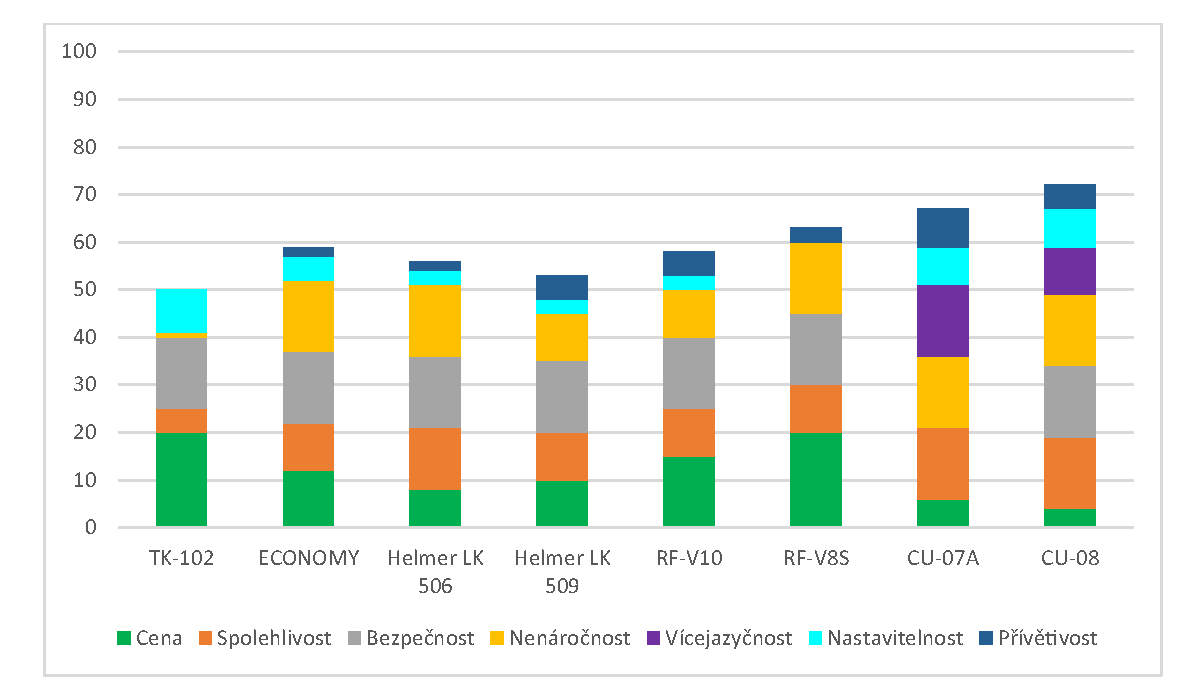
\includegraphics[width=\textwidth]{graphs/graf_bodoveHodnoceni.pdf}
\caption{Grafické znázornění bodového hodnocení dostupných modelů}
\label{image}
\end{center}
\end{figure}

% Koncept

\chapter{Koncept}
Při tvorbě konceptu jsem se zaměřil na výběr obecných součástek, nespecifikuji tedy konkrétní výrobky, ale pouze jejich typ, díky čemuž není koncept svázán s určitým výrobkem a kusy lze nahradit jinými, které budou fungovat stejným způsobem. Dále jsem zvolil, jak budou součástky propojeny, cestu, kterou budou komunikovat a čím budou napájeny.

\section{Řídící jednotka}
Základem celého sledovacího zařízení je řídící jednotka, která ovládá veškeré dění, přijímá a zpracovává data, která následně vyhodnocuje. Na základě požadovaných vlastností jsem se rozhodl pro mikrokontrolér, který je integrovaným obvodem, tedy v základní struktuře obsahuje procesor, operační paměť, paměť pro program, oscilátor, vstupní a výstupní rozhraní (porty). Volbu jsem učinil zejména z hlediska nízké ceny a dostačujících parametrů. Mikrokontroléry se vyznačují velmi vysokou spolehlivostí, kompaktnostní a nízkou cenou, která je mým cílem. Často jsou využívány pro jednoúčelové aplikace řízení, nebo regulace.

\section{Komunikační rozhraní}
Komunikační rozhraní je zařízení, které poskytuje přístup do sítí GSM, GPS a popřípadě GPRS. Rozraní může obsahovat více komunikačních čipů, například jeden pro GPS, druhý pro GSM a tím umožní komunikaci v obou sítích zároveň. Nebo pomocí jednoho čipu, který kombinuje všechny sítě do jednoho zařízení, ale není možná komunikace ve více sítích zároveň, je tedy nutné mezi nimi přepínat. Rozraní musí poskytovat jednoduché příkazy, které umožní komunikovat přes zmíněné sítě, bez potřebné znalosti jejich interní struktury. Bude tedy možné pomocí jednoduchého příkazu odeslat zprávu SMS, nebo bude poskytovat data z GPS ve specifickém formátu, který bude možné zpracovat a vyhodnotit.

\section{Senzor pohybu}
Pro notifikaci změny pohybu a maximální úsporu elektrické energie je nutné sledovací zařízení opatřit senzorem pohybu. Jedná se o čidlo, které zaznamenává změnu své vlastní polohy, nejedná se tedy o detektor pohybu, který zaznamenává pohyb okolí. Pro koncept je možné využít vibrační senzor, je levný (desítky korun), nepřesný (nelze nastavit přesnost) a používá jej většina dostupných modelů. Vibrační senzor má nulovou spotřebu, protože se jedná o drátek uvnitř pružinky, která se ho v případě pohybu dotkne a uzavře se elektrický okruh. Dále je možné použít akcelerometr, který z porovnávaných modelů mají pouze modely od firmy Jablotron. Senzor je dražší (stovky korun) ale na druhou stranu je přesný (lze nastavit přesnost), spotřeba je u většiny modelů 10 mA. Možným řešením by byla detekce pohybu pomocí změny polohy GPS, nicméně spotřeba při připojení do sítě GPS se pohybuje kolem 200 mA, proto toto řešení označuji jako nevhodné, vzhledem k jeho nárokům na energii.

\section{Napájení}
Jako napájení může být použita autobaterie, nebo jakýkoliv jiný zdroj energie o minimálním napětí 12 V a minimálním výstupním proudem 1 A. Vstupní napětí 12 V je minimální potřebné napájecí napětí, které vyžaduje komunikační modul. Maximální velikost vstupního napětí bude dána použitým regulátorem napětí, který sníží vyšší napětí na požadované. Proudový odběr 1 A je maximální možný odběr, který bude zařízení schopno vyvinout. Při použití zdroje napájení s nižším maximálním proudem, než 1 A, může dojít k poklesu napětí, nebo nenávratnému poškození zdroje napájení (baterie), pokud je proud, které zařízení zrovna potřebuje vyšší, než proud který je zdroj napájení schopen dodat. Poškozením je myšleno roztavení a v některých případech i explozi (dle typu baterie). Mezi sledovací zařízení a zdroj napájení, bude umístěna vratná pojistka (PolySwitch), která ochrání sledovací zařízení před nadproudem či zkratem. 

\section{Blokové schéma}
Blokové schéma ukazuje propojení jednotlivých částí do funkčního celku. Zdroj napájení je přes vratnou pojistku napojen na řídící jednotku, která dále rozděluje energii mezi další součástky, dle jejich potřeb (12 V, 5 V, 3 V). Řídící jednotka má na sebe napojen senzor pohybu, který indikuje změny pohybu a v případě změny, řídící jednotku probudí ze spánku. Na řídící jednotku je také napojeno komunikační rozhraní, které pouze vykonává příkazy řídící jednotky, popřípadě jí zasílá příchozí data. Dle typu komunikačního rozhraní je napojen na síť GPS, GSM, popřípadě GPRS.

\begin{figure}[H]
\begin{center}
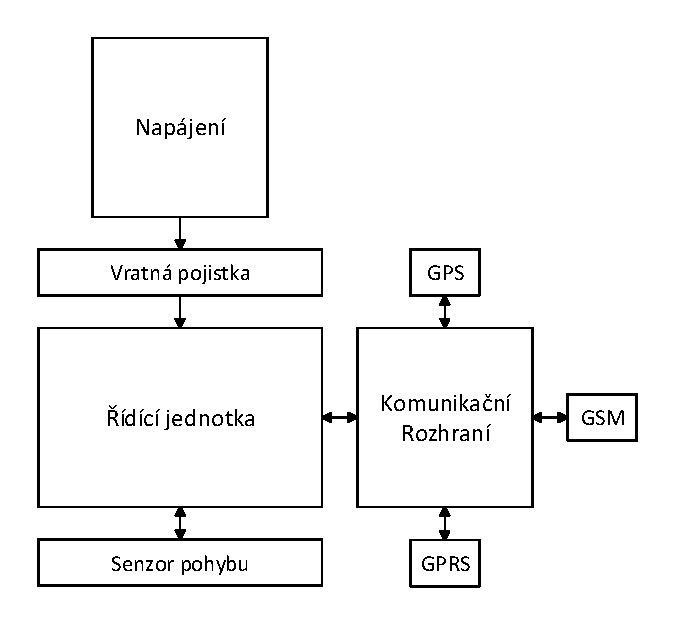
\includegraphics[width=\textwidth]{graphs/schema_blokove.pdf}
\caption{Blokové schéma zapojení}
\label{image}
\end{center}
\end{figure}

% Prototyp

\chapter{Prototyp}
Před tvorbou prototypu jsem se s vedoucí práce dohodl na využití hotových dílů, které poskládám dohromady a naprogramuji. Cílem této práce není vytvoření sledovacího zařízení, připraveného do sériové výroby, ale vytvoření prototypu na kterém ukáži zvolené hardwarové a softwarové řešení.

\section{Vývojová deska Arduino}
Jako řídící jednotku jsem si zvolil vývojovou desku Arduino UNO \cite{Arduino schematic} od společnosti Arduino, která obsahuje čip ATmega328 \cite{Atmega datasheet}. Možnosti čipu i desky mnohonásobně přesahují požadavky na výkon i periferie, nicméně díky jednoduchému programování desky \cite{Pruvodce arduinem}, bude možný rychlý vývoj řídícího softwaru. V případě finální výroby navíc počítám s pouze jednodušší variantou čipu ATmega, takže finální kód by zůstal stejný. ATmega i jiná řešení jsou programována v jazyce C, tedy není problém s výměnou čipu za jiné řešení, pouze by bylo nutné upravit některé příkazy pro určitý čip. Čip řady ATmega používá jazyk C s vývojovou platformou Wiring.

\begin{figure}[H]
\begin{center}
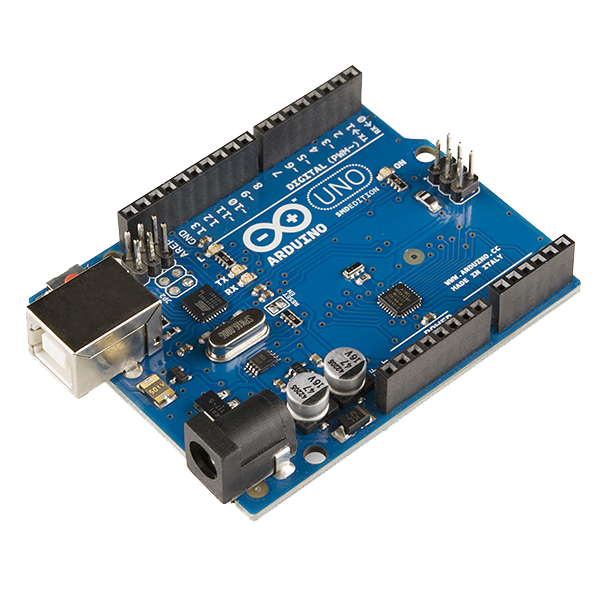
\includegraphics[width=0.5\textwidth]{images/arduino.png}
\caption{Vývojová deska Arduino UNO}
\label{image}
\end{center}
\end{figure}

\section{Komunikační modul GPS/GPRS/GSM}
Komunikační modul jsem volil tak, aby byl kompatibilní s Arduinem, díky čemuž se zjednoduší propojení a umožní komunikačním modulem přímo rozšířit vývojovou desku Arduino. To nastane jednoduchým nasazením na desku, kdy jsou nožičky (piny) obou zařízení propojeny. Zvolil jsem řešení GPS/GPRS/GSM Module V3.0 \cite{ROBOT schematic} od firmy DFROBOT, které obsahuje možnost jednoduchého připojení všech možných periferií (mikrofon, reproduktor, sim karta atd.), čímž je skvělým modulem pro testování a vývoj. Hlavní částí je komunikační čip SIM908 \cite{SIMCOM HW}, který umí komunikovat přes GPS, GSM i GPRS a navíc je jednoduše ovladatelný \cite{SIMCOM SW}. Čipy řady SIM900 jsou využívány ve všech nalezených sledovacích zařízeních, jedná se o jedno z mála dostupných řešení, které je levné a v případě budoucí výroby předpokládám jeho použití, proto bude software postaven na komunikaci s tímto čipem.

\begin{figure}[H]
\begin{center}
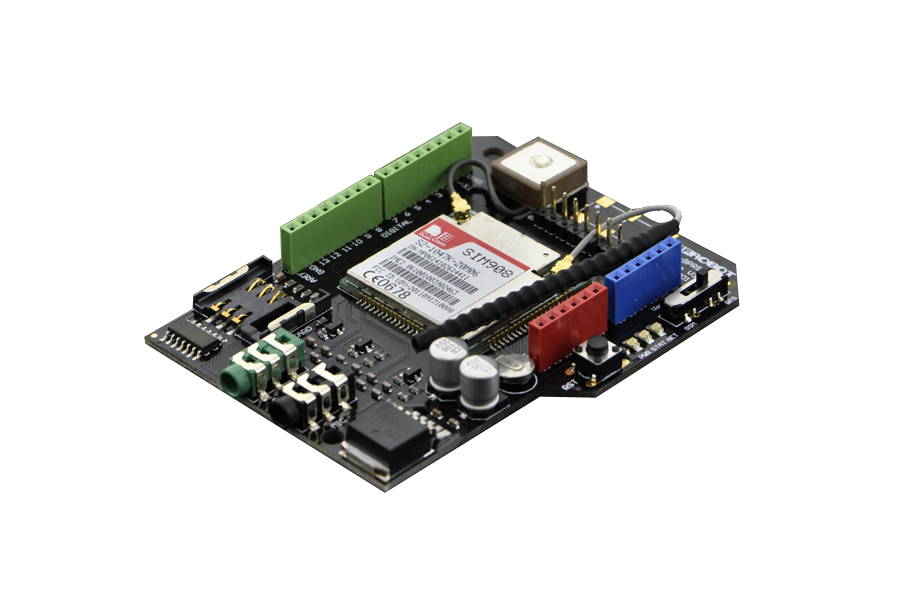
\includegraphics[width=0.8\textwidth]{images/module.png}
\caption{Komunikační modul GPS/GPRS/GSM Module V3.0}
\label{image}
\end{center}
\end{figure}

\section{Akcelerometr}
Senzorem pohybu jsem zvolil desku GY-521 s čipem MPU-6050, který obsahuje akcelerometr a gyroskop v jednom. Pro tento akcelerometr jsem se rozhodl, protože je plně podporován a otestován pro desku Arduino \cite{Arduino acce}, navíc existuje velké množství oficiálních článků a knihoven \cite{I2cdevlib} pro jeho ovládání. Čip komunikuje přes sběrnici I2C, která díky modelu master/slave umožňuje připojit více různých i stejných zařízení. Velkou výhodou je také programovatelný čip, který může v případě potřeby desku Arduino probudit ze spánku, nebo provádět jakékoliv výpočty.

\begin{figure}[H]
\begin{center}
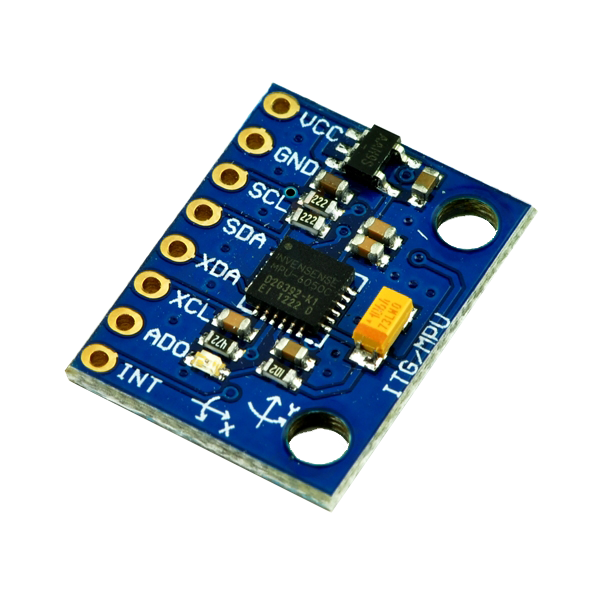
\includegraphics[width=0.5\textwidth]{images/akcelerometr.png}
\caption{Akcelerometr GY-521 s čipem MPU-6050}
\label{image}
\end{center}
\end{figure}

\section{Náklady na prototyp}
Pro úplnost informací o prototypu, přikládám tabulku s informacemi, odkud byla součástka zakoupena, kdy byla obdržena a za jakou cenu. Oproti vyjmenovaným součástkám výše, je navíc v seznamu také vratná pojistka PolySwitch, která byla zmíněna v blokovém zapojení, dále napájecí adaptér pro účely vývoje mimo vozidlo a k němu příslušný napájecí kabel, který není standardní součástí adaptéru. Všechny součástky byly objednány dne 11. 1. 2016 z internetu a vyzvednuty na pobočkách.

\renewcommand{\arraystretch}{1.5}
\begin{table}[H]
\begin{center}
\begin{tabular}{| l | c | c | r |}
\hline
Položka & Obchod & Obdržení & Cena s DPH\\
\hline
\hline
Arduino UNO R3 & GME & 13.1.2016 & 665 Kč\\
\hline
GPS/GPRS/GSM Shield V3 & GME & 14.1.2016 & 2 270 Kč\\
\hline
Vratná pojistka PolySwitch 3A & GME & 13.1.2016 & 15 Kč\\
\hline
Napájecí síťový adaptér 12V/3A & GME & 13.1.2016 & 330 Kč\\
\hline
Napájecí síťový kabel & GME & 13.1.2016 & 42 Kč\\
\hline
Akcelerometr GY-521 & Arduino-Shop & 16.1.2016 & 150 Kč\\
\hline
\hline
\multicolumn{3}{| l |}{Doprava celkem} & 245 Kč\\
\hline
\hline
\multicolumn{3}{| l |}{Cena celkem} & 3 717 Kč\\
\hline
\end{tabular}
\end{center}
\caption{Náklady na stavbu prototypu}
\end{table}

%Softwarový návrh

\chapter{Softwarový návrh}
V programové části se nejdříve zaměřím na popis programovacího jazyka, vývojové prostředí, ve kterém bude software tvořen a dále na postupy při tvorbě jednotlivých částí, problémy se kterými jsem se u nich setkal a jakým způsobem jsem je vyřešil.

\section{Programovací jazyk}
Vývoj softwaru bude probíhat v programovacím jazyce C s nadstavbou vývojové platformy Wiring  (knihovna Wire)\cite{Arduino acce}, která jazyk rozšiřuje o nové příkazy, pro přímé řízení hardwarových součástek, vše zastřešeno sadou knihoven \cite{Arduino lib} (od tvůrců desky Arduino), které přidávají nové funkce, aby potencionální vývojář nepotřeboval hlubší znalosti programování a hardwaru. Tento kompletní balík příkazů \cite{Arduino lang} je někdy také nazýván programovacím jazykem Arduino \cite{Arduino intro}.

\section{Vývojové prostředí Arduino}
Pro vývoj softwaru budu používat oficiální vývojové prostředí, od tvůrců desky Arduino s identickým názvem Arduino \cite{Arduino soft}. Jedná se o počítačový software s otevřeným zdrojovým kódem (open-source) \cite{Arduino source}, určený k jednoduchému psaní a nahrávání zdrojových kódů na desku. Prostředí lze nainstalovat na operační systém Windows, MAC a Linux. Z vlastní zkušenosti vyjmenuji výhody, mezi které patří zvýraznění a barevné rozlišení jednotlivých příkazů, plná podpora vývojové platformy Wiring, podpora všech oficiálních i neoficiálních desek Arduino, zabudovaný klient pro komunikaci na sériové lince a dalších funkce. Nevýhodou je absence předvídání a dokončování kódu (predikce), nápověda při volání částí programu (funkcí, knihoven atd.), nemožnost krokování programu a velice obecné chybové hlášky, kvůli kterým je náročné odhalit případné chyby.

\begin{figure}[H]
\begin{center}
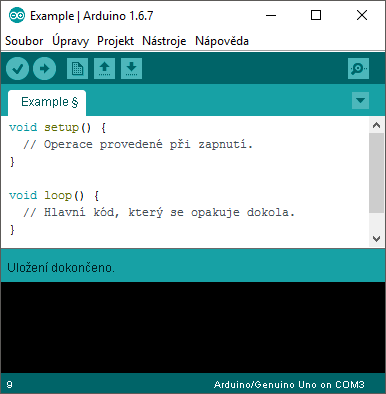
\includegraphics[width=0.8\textwidth]{images/arduino-ide.png}
\caption{Ukázka z vývojového prostředí Arduino}
\label{image}
\end{center}
\end{figure}

% Hlavní program

\section{Hlavička programu}
V hlavičce jsou definovány všechny globální proměnné, které jsou určeny primárně ke změnám pomocí příkazů SMS. Především se ale v této části nachází textové řetězce, které jsou na jednom uceleném místě, určené například k jednoduchému rozšíření do jiného jazyka, nebo k úpravám již stávajících testových řetězců.

\section{Hlavní funkce programu}
Pod hlavičkou programu se nachází zdrojové kódy, které tvoří jádro celého programu, hlavními částmi jsou inicializace (setup), která slouží pro uvedení do výchozího stavu a smyčka (loop), která dle situace volá ostatní podprogramy (funkce). Níže detailně popíši všechny funkce hlavního programu, jaký je jejich účel, jaké mají vstupní parametry a co je jejich výstupem.

\subsection{Inicializace (setup)}
Inicializace slouží k uvedení zařízení do výchozího stavu a načtení nastavení a dat z paměti. Jako první se nastaví všechny piny, které se budou používat jako výstupní, dále se všechny piny, používané pro signalizace diodamy LED, nastaví do logické nuly. Je zahájen komunikační rámec seriové linky, pro komunikaci s modulem GPS/GSM/GPRS, popřípadě s počítačem, který slouží pro monitorování stavu.  Následuje přepnutí řídících pinů do logické jedna, které znamenají, aby se modul připojil do sítě. Nakonec je zařízení přepnuto do režimu GSM, zavoláním funkce changeMode, s textovým parametrem GSM. Funkce pracuje pouze s globálními proměnnými a nevrací žádný výstup.

\subsection{Hlavní smyčka (loop)}
Hlavní smyčka je jádrem, které spojuje všechny funkce do jednoho celku, zastřešuje jejich funkčnost a zajištuje vzájemnou provázanost. Kód je rozdělen na části podle režimu modulu, pokud je v režimu GSM, čeká na příchozí komunikaci. Pokud jí obdrží, načte kompletně jeden komunikační rámec a poté ověří, zda se jedná o SMS, pokud ano, jsou volány postupně další funkce, které načtou hlavičku, obsah a nakonec požadavek v obsahu těla SMS vykonají. Druhá část je částí GPS, kdy se čeká pouze na plně načtená data z přerušení. Pokud jsou data kompletní, začne zpracování a výpočet validních dat GPS, pokud jich je dostatek a je ověřena jejich validita, je modul přepnut do režimu GSM a předá mu informace o poloze. Funkce pracuje pouze s globálními proměnnými a nevrací žádný výstup.

\subsection{Rozpoznání chyb (recognizeERROR)}
Funkce byla navržena po zjištění příčiny náhodných pádů a zamrznutí modulu. Modul se náhodně vypínal, přestal komunikovat, nebo jednoduše ztratil spojení. Po důkladném průzkumu dokumentace \cite{ROBOT SW} jsem odhalil, že příčinou může být několik věcí, v čele s nestabilním napájením. Pokud takováto situace nastane, modul vyšle příznak označený jako NORMAL POWER DOWN a přestane odpovídat. V dokumentaci je řečeno, že jediný způsob jak vzpamatovat zařízení z chyby, je ruční restart Arduina i modulu samotného. Restart modulu, ani Arduina, nelze provést standardní cestou. Existují dvě možnosti, z nichž jedna méně elegantní, je propojení vybraného pinu s pinem reset, při sepnutí se celé zařízení restartuje. Druhé elegantnější řešení, které jsem zvolil, je externí knihovna pro softwarový restart. Z oficiálních stránek Arduino, jsem nalezl jsem knihovnu SoftReset \cite{SoftReset} s volně šířítelným zdrojovým kódem, kterou jsem vnořil do svého kódu. Nyní, když dorazí příznak NORMAL POWER DOWN, jsou uložena stávající data a zařízení restartována. Poté pokračují tam, kde naposledy skončila. Funkce pracuje pouze s globálními proměnnými a nevrací žádný výstup.

\subsection{Odešli příkaz do modulu (sendCommand)}
Jednořádková funkce, sloužící k odeslání příkazu do modulu. Slouží pouze k jednoduché změně názvu sériového portu pro komunikaci se zařízením. Pokud by byl v celém kódu používán příkaz osamoceně, bylo by při změně názvu portu nutné ruční přepsání všech výskytů v kódu. Jednoduchým vnořením do této funkce, stačí název zařízení změnit pouze zde a neovlivní to zbytek programu. Obdržený textový řetězec funkce pošle přes sériovou linku k předem definovanému zařízení.

\paragraph{Vstupní parametr funkce:}
\begin{itemize}
\item textový řetězec String s kompletním příkazem pro modul.
\end{itemize}

\subsection{Odešli zprávu o stavu do PC (sendReport)}
Jednoduchá funkce, v případě režimu ladění (lze zapnout v hlavičce), odesílá informace o veškerém dění do připojeného počítače. Na vstupu obdrží textový řetězec, který pouze po seriové lince pošle do předem definovaného zařízení. Funkce je volána z částí kódu, kde je prováděna jakákoliv významná operace a jedná se o jediný možný způsob ladění. Funkce nevrací žádný výstup.

\paragraph{Vstupní parametr funkce:}
\begin{itemize}
\item textový řetězec String se zprávou o tom, co program vykonává v tuto chvíli.
\end{itemize}

\subsection{Změň režim modulu (changeMode)}
Funkce slouží k přepínání režimů modulu a celkově práce kterou provádí řídící jednotka. Aktuálně podporuje pouze přepínání mezi režimy GSM a GPS, je ale jednoduše rozšířitelná o další režimy, které nemusí být pouze záležitostí modulu, ale i vnitřních pochodů. Po rozpoznání vstupního parametru se provedou procedury, potřebné k přepnutí do druhého režimu, ty jsou definovány v softwarové dokumentaci komunikačního čipu \cite{SIMCOM SW}, osazeném na modulu. Funkce pracuje s globálními proměnnými a nevrací žádný výstup.

\paragraph{Vstupní parametr funkce:}
\begin{itemize}
\item textový řetězec String s režimem, do kterého má být modul přepnut.
\end{itemize}

% Režim GSM

\section{Funkce v režimu GSM}
Níže detailně popíši všechny funkce režimu GSM, jaký je jejich účel, jaké mají vstupní parametry a jaká je jejich návratová hodnota.

\subsection{Rozpoznání nové SMS (recognizeSmsNew)}
Funkce obstarává zjištění, zda v režimu GSM dorazila nová SMS, to dává modul navědomí textovým řetězcem +CMTI, viz softwarová dokumentace \cite{SIMCOM SW}. Po registrování nové SMS je modulu zaslána žádost AT+CMG=1 \cite{SIMCOM SW}, která slouží k vyžádání hlavičky a těla textové zprávy. Funkce pracuje s globálními proměnnými a nevrací žádný výstup.

\subsection{Rozpoznání hlavičky SMS (recognizeSmsHeader)}
Pokud byla obdržena nová SMS, očekává se přijetí, její hlavičky. Pokud tak nastane, je z hlavičky vyčteno telefonní číslo odesílatele, na které bude později odeslána odpověď SMS. Číslo je uloženo do globální proměnné a je nastaven příznak čtení SMS, tedy značí, že je program připraven číst obsah. Funkce pracuje pouze s globálními proměnnými a nevrací žádný výstup.

\subsection{Rozpoznání obsahu SMS (recognizeSmsContent)}
Po rozpoznání hlavičky SMS a nastavení příznaku čtení, je očekáván obsah zprávy. Modul posílá zprávu ihned po hlavičce, ale v případě, že by se tak nestalo, proběhne ověření, zda se opravdu jedná o zprávu SMS zkontrolováním obsahu zprávy, zda není prázdný (znak nového řádku vždy chodí před příkazem) a zda je nastaven příznak čtení. Poté jsou příchozí data vyčtena a označena za tělo zprávy SMS. Funkce pracuje pouze s globálními proměnnými a nevrací žádný výstup.

\subsection{Vykonání obsahu SMS (executeSmsContent)}
V případě, že je zpráva kompletní, je zavolána funkce pro vykonání obsahu SMS. Zde je textový řetězec ve zprávě SMS, dle jazyka, porovnáván s textovými řetězci v globálních proměnných, kde se ověřují pouze znaky, nezáleží tedy zda jsou písmenka malá, nebo velká. Pokud obsah sedí do jednoho z definovaných textů, je vykonán požadavek. Například pokud bude přijata zpráva \uv{Kde jsi?}, bude obratem odeslána odpověď: \uv{Probíhá lokalizace, poloha bude zaslána během několika minut}, odesláním textu do funkce sendSMS(), následně je modul přepnut do režimu GPS a tím ukončena činnost této části kódu. Funkce pracuje pouze s globálními proměnnými a nevrací žádný výstup.

\subsection{Odeslání SMS (sendSMS)}
Funkce přepne modul do textového režimu, bude tedy očekávat odeslání textového řetězce, dále odešleme informaci pro odeslání SMS na telefonní číslo, uvedeném v příkazu. Čekáme na odpověď, když dorazí, je modul v režimu přijímání textu a jeho ukončení je možné pouze kombinací kláves CTRL+C, tato klávesová zkratka má naštěstí svou hodnotu v tabulce ASCII, tedy hodnotu 42. Funkce odešle všechen text, který obdržela na vstupu v textovém řetězci, poté je odeslán ukončovací příznak CTRL+C. Tím je SMS zpráva úspěšně odeslána do modulu, který již dále převezme režii, separovaně od úloh řídící jednotky. Mezi každým krokem jsou nastaveny časové intervaly, definované v hlavičce, které slouží jako doba, kterou má modul na odpověď našeho požadavku. Funkce nevrací žádný výstup.

\paragraph{Vstupní parametr funkce:}
\begin{itemize}
\item textový řetězec String se zprávou SMS.
\end{itemize}

% Režim GPS

\section{Funkce v režimu GPS}
Níže detailně popíši všechny funkce režimu GPS, jaký je jejich účel, jaké mají vstupní parametry a jaká je jejich návratová hodnota.

\subsection{Obsluž přerušení (serialEvent)}
V režimu GPS není možné vyčítat data ze sběrnice dle libosti, paměť, do které se ukládají data, má své limity a při zahlcení se začnou data přemazávat, jediným řešením je včasné čtení dat, čímž se z paměti smažou a uvolní své místo. V režimu GPS přijde jeden balík dat za méně než 1 s, proto jsou data vyčítána přerušením, aby se nemuselo čekat na obsloužení dalších částí kódu. Pokud existují příchozí data, je vyvoláno hardwarové přerušení, které aktivuje funkci serialEvent(), ta dokud jsou data v paměti, vyčítá do jednoho textového řetězce a po vyprázdnění paměti odešle data ke zpracování, vztyčením příznaku stringComplete. Funkce pracuje s globálními proměnnými a nevrací žádný výstup.

\subsection{Vyčti údaje o poloze z dat (parseCoordinates)}
Příchozí data musí být zpracována a vyčteny z nich pouze důležité informace. Data jsou ve formátu NMEA specifikované v původní dokumentaci od společnosti SIFT TECHNOLOGY \cite{SIFT}, nebo v novější verzi od společnosti CSR PLC \cite{CSR}, která původní společnost odkoupila. Informace jsem čerpal z obou oficiálních dokumentací. Z jednoho komunikačního rámce jsou vyjmuty hodnoty zeměpisné šířky a délky, která jsou následně odeslána k převodu na přesné souřadnice. Funkce pracuje pouze s globálními proměnnými a nevrací žádný výstup.

\subsection{Oprava souřadnice (gpsCorrection)}
Dlouhé týdny jsem se zabýval problémem, že zjištěná poloha nebyla nikdy přesná. Přesněji se od skutečné lišila od 100 do 1 000 m. V oficiální dokumentaci ani v podkladech nic takového psáno nebylo, ale našel jsem diskusi na internetovém fóru \cite{correct}, kde se problém podařil dvou uživatelům vyřešit. Na základě jejich poznatků a algoritmů jsem jejich postup implementoval do svého zdrojového kódu. Po aplikování algoritmu se přesnost zpřesnila na jednotky metrů.

\paragraph{Vstupní parametr funkce:}
\begin{itemize}
\item float s hodnotou polohy
\end{itemize}

\paragraph{Návratová hodnota funkce:}
\begin{itemize}
\item float s opravenou hodnotou polohy
\end{itemize}

\subsection{Počítej validní GPS (countValidGpsCoordinates)}
Pro zjištění, zda je pozice validní, jsem použil všebecně dostupné infomace o polohování na planetě Zemi \cite{geographic}, podle kterých jsem vymezil hodnotám určité hranice, kterých mohou nabývat. Pokud jsou souřadnice v pořádku, jsou připočteny do validních dat, kterých, pokud je určitý počet, definovaný v hlavičce, jsou pak označena jako validní poloha a ta je připravena k dalšímu zpracování, například odeslání. Je nutné zmínit, že pokud jsou příchozí data z modulu poškozená nebo nevalidní, jsou při převodu z formátu String (textový řetězec) do formátu Float (číslo s desetinou čárkou) označena jako nevalidní a funkce .toFloat() vrací hodnotu nula, tedy pokud jsou souřadnice nulové, není poloha platná. Nulové souřadnice ale existují, nachází se na jihozápad od Afriky, nicméně nepředpoládám že by se sledovací zařízení do tohoto místa dostalo. Pokud ano, nebude se jistě zdržovat přesně na poloze o souřadnicích [0;0]. Tento nedostatek bude při potencionálním budoucím vývoji odstraněn. Funkce pracuje pouze s globálními proměnnými a nevrací žádný výstup.

% Ukázka komunikace
\section{Ukázka komunikace}
Obrázek níže zobrazuje, jak může vypadat komunikace mezi uživatelem, který zjišťuje, kde se sledovací zařízení nachází a samotným zařízením, které na žádost odpovídá. Následně zasílá výslednou polohu, ve formě odkazu s mapy Google. Celá komunikace probíhá formou psaného slova, příkazy jsou tedy pro uživatele přívětivější a lépe zapamatovatelné.

\begin{figure}[H]
\begin{center}
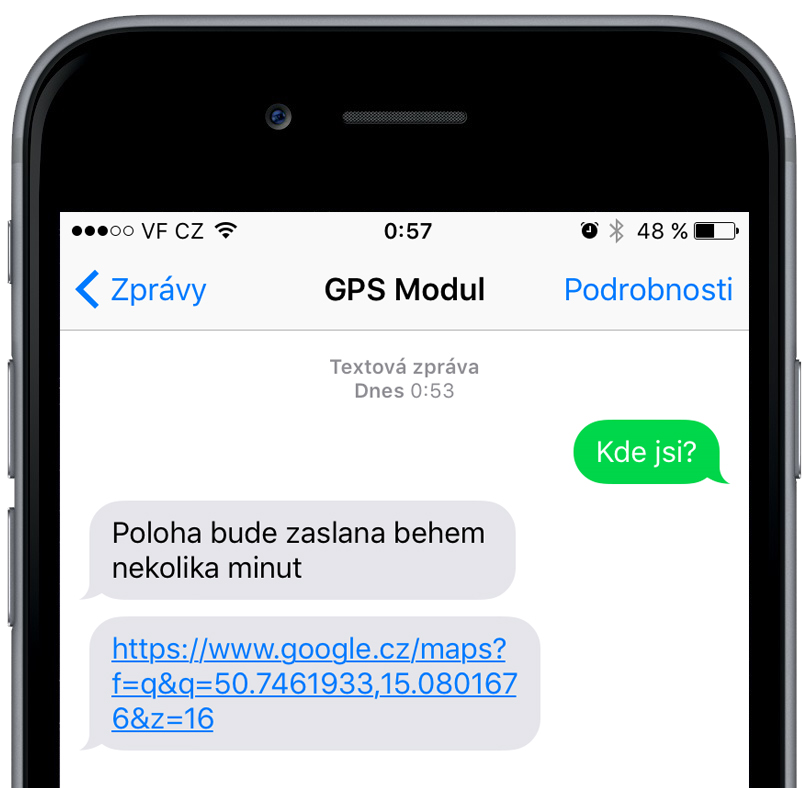
\includegraphics[width=0.6\textwidth]{images/comm.png}
\caption{Příklad komunikace se sledovacím zařízením}
\label{image}
\end{center}
\end{figure}

% Spotřeba

\chapter{Spotřeba a výdrž na autobaterii}
Hotový prototyp jsem po otestování podrobil měření spotřeby, ve všech možných režimech. Měření probíhalo při pokojové teplotě 22 \degree C, výsledky jsou zobrazeny v tabulce níže. Z naměřených veličin jsem vypočetl teoretickou výdrž v hodinách, podle vzorečku níže, výsledky zanesl do tabulky a následně je převedl na výdrž ve dnech, pro lepší představu. Hodnoty jsem také zanesl do tabulky. Při výpočtech počítám se slabší autobaterií o kapacitě 50 Ah, nicméně se běžně používají silnější. Dny jsou zaokrouhlovány vždy dolů, na celý jeden den. Z vypočtených hodnot vyplývá, že zařízení teorieticky vydrží na nedobíjenou autobaterii přibližně 30 dnů a při správné implementaci zdrojových kódů akcelerometru, do zdrojových kódů řídící jednotky, které jsem již zhotovil, je možné dosáhnout teoretické vypočtené výdrže až 200 dní. V případě vybité baterie, by bylo vhodné notifikovat o tomto stavu majitele zařízení.

\paragraph{Použíté měřící přístroje:}
\begin{itemize}
\item stabilizovaný zdroj napětí Tesla-BS 525
\item osciloskop HUNG CHANG 3502 20 MHz
\item digitální multimetr DT9205A
\end{itemize}

\paragraph{Výpočet výdrže z naměřené spotřeby:}
$$ vydrz [hodin] = \frac{1}{\frac{spotreba[mA]}{1000}} \times autobaterie[Ah] $$

\renewcommand{\arraystretch}{1.5}
\begin{table}[H]
\begin{center}
\begin{tabular}{| l | c | c |  c |}
\hline
Režim & Naměřená spotřeba & Výdrž [hodiny] & Výdrž [dny]\\
\hline
\hline
GSM & 150 mA & 333 & 13\\
\hline
GPS & 200 mA & 250 & 10\\
\hline
Arduino & 60 mA & 833 & 33\\
\hline
Akcelerometr & 10 mA & 5000 & 200\\
\hline
\end{tabular}
\end{center}
\caption{Naměřená spotřeba a vypočtená výdrž v hodinách a dnech}
\end{table}

% Bodové hodnocení vlastního řešení

\chapter{Bodové hodnocení vlastního řešení}
Stejnou metodikou jako u konkurenčních výrobků, jsem zhodnotil vlastnosti svého vlastního zařízení, které bylo stavěno tak, aby dosáhlo maximálního počtu bodů ve všech kategoriích. Cílové zařízení bylo postaveno ze součástek, díky nimž bude možné cenu udržet do hodnoty 1 000 Kč včetně teoretické výroby a zbývá tedy velký prostor pro zisk a cenově se stále drží v kategorii nízkonákladových zařízení (20). Řešení je kvalitně softwarově i hardwarově zpracováno, nicméně chybí druhý komunikační čip, který by zajistil 100\% dostupnost v obou sítích zároveň (10). Umístěním u autobaterie, která zařízením v této kategorii chybí, se zařízení stává špatně odhalitelným (15) a malá výdrž zajišťuje minimální nároky na energii autobaterie (15). Jazykové možnosti jsou neomezené, nicméně zatím chybí překlad textových řetězců (12). Možnosti nastavení jsou obrovské a snadno rozšířitelné (10) a komunikace probíhá v běžné řeči, zařízení je tedy jednoduše ovladatelné a uživatelsky přívětivé (10). (Celkem 92 bodů)

\paragraph{Bodové ohodnocení vlastního řešení:}
\begin{itemize}
\item cena (20 bodů)
\item spolehlivost (10 bodů)
\item bezpečnost (15 bodů)
\item nenáročnost (15 bodů)
\item vícejazyčnost (12 bodů)
\item nastavitelnost (10 bodů)
\item přívětivost (10 bodů)
\end{itemize}

\renewcommand{\arraystretch}{1.5}
\begin{table}[H]
\begin{center}
\begin{tabular}{| l | c | c| c | c | c | c | c | c |}
\hline
Název sledovacího zařízení & CE & SP & BE & NE & JA & NA & PŘ & Celkem\\
\hline
\hline
Vlastní řešení & 20 & 10 & 15 & 15 & 12 & 10 & 10 & 92\\
\hline
TK-102 & 20 & 5 & 15 & 1 & 0 & 9 & 0 & 50\\
\hline
ECONOMY & 12 & 10 & 15 & 15 & 0 & 5 & 2 & 59\\
\hline
Helmer LK 506 & 8 & 13 & 15 & 15 & 0 & 3 & 2 & 56\\
\hline
Helmer LK 509 & 10 & 10 & 15 & 10 & 0 & 3 & 5 & 53\\
\hline
RF-V10 & 15 & 10 & 15 & 10 & 0 & 3 & 5 & 58\\
\hline
RF-V8S & 20 & 10 & 15 & 15 & 0 & 0 & 3 & 63\\
\hline
CU-07A & 6 & 15 & 0 & 15 & 15 & 8 & 8 & 67\\
\hline
CU-08 & 4 & 15 & 15 & 15 & 10 & 8 & 5 & 72\\
\hline
\end{tabular}
\end{center}
\caption{Bodové hodnocení dostupných modelů a vlastního řešení}
\end{table}

\begin{figure}[H]
\begin{center}
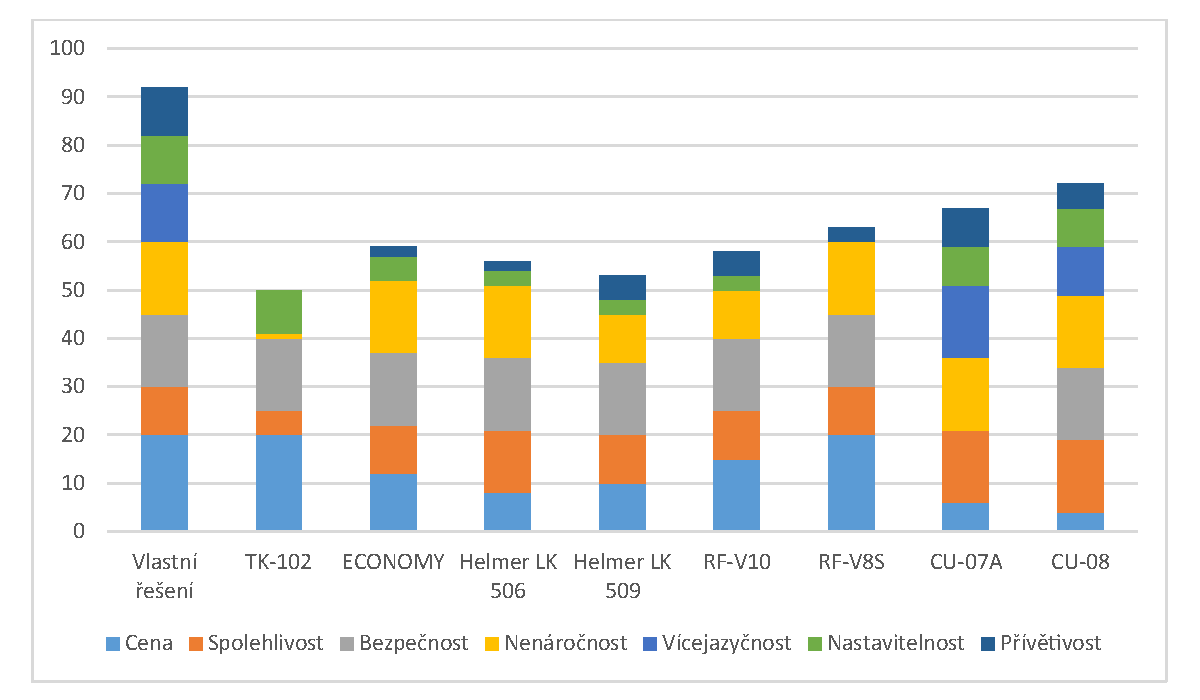
\includegraphics[width=\textwidth]{graphs/graf_bodoveHodnoceni_final.pdf}
\caption{Grafické hodnocení vlastního řešení a dostupných modelů}
\label{image}
\end{center}
\end{figure}

% Závěr

\chapter{Závěr}
V rešeršní části jsem definoval sledovací zařízení, seznámil jsem se s jeho historií i současností a definoval jsem vlastní požadované vlastnosti, které pro mě hrají důležitou roli při tvorbě zmíněného zařízení. Nakonec jsem se seznámil s platnými standardy a technickými předpisy související s tématem práce. Průzkumem trhu jsem vytvořil kategorie sledovacích zařízení, dle jejich cenových hladin a vlastností těmto hladinám vlastním. Definoval jsem ideální nízkonákladové zařízení, kdy jsem každé požadované vlastnosti přiřadil maximální počet bodů a poté jsem vyhodnotil nejkvalitnější, mnou vybrané konkurenční výrobky, kterým jsem udělil příslušný počet bodů v každé kategorii, kdy zařízení s nejvyšší cenou získalo nejvyšší počet bodů (72/100) a zařízení s cenou nejnižší, získalo bodů nejméně (50/100).

Na základě častých konzultací s vedoucí práce, jsem navrhl koncept cílového zařízení, doporučil realizační postupy, vybral hardware, nebo uvedl více možností jeho výběru, kterými může být dosaženo výsledného zařízení. Následně jsem zvolil komunikační prostředky a architekturu jednotlivých komponentů. Nakonec jsem pro koncept vybral vhodné osazení ve voze a vytvořil blokové zapojení komponentů. Vše jsem pečlivě vybíral tak, aby byla výrobní cena co nejnižší, nejlépe aby se držela pod hranicí 1 000 Kč, ale vlastnosti dosahovaly ideálního sledovacího zařízení.

Na základě konceptu jsem zvolil nejvhodnější komponenty pro vývoj prototypu, které jsem následně zakoupil. Nastudoval jsem použitý programovací jazyk, včetně knihoven, které jsem později použil ve svém kódu. Před psaním kódu jsem popsal programové prostředí, ve kterém bude vývoj probíhat, po dopsání vlastního kódu jsem podrobně popsal všechny funkce programu, jejich možnosti, vlastnosti, vstupní parametry a návratové hodnoty. 

Funkční prototyp jsem otestoval v běžném provozu, kdy 14 dní nepřetržitě běželo bez jediného pádu či problému a poté jsem testování ukončil. Dále jsem změřil spotřebu jednotlivých komponentů i celého zařízení a naměřil teoretickou výdrž až 200 dní nepřetržitého provozu, při použití s nejslabší používanou autobaterii o kapacitě 50 Ah, která po celou dobu nebude dobíjena.

Nakonec jsem své zařízení ohodnotil stejnou metodikou, kterou jsem použil pro hodnocení konkurenčních výrobků, přičemž mé sledovací zařízení získalo 92 bodů.

Vývoj sledovacího zařízení má před sebou ještě dlouhou cestu do finální podoby, ale věřím, že v práci budu pokračovat a vše dokončím dle mých původních představ.

\addcontentsline{toc}{chapter}{Literatura}
\begin{thebibliography}{10}
\bibitem{guide}A Guide To The Global Positioning System. Radioshack [online]. [cit. 2016-05-09]. Dostupné z: \url{http://support.radioshack.com/support\_tutorials/gps/gps\_tmline.htm}
\bibitem{Arduino intro}Arduino introduction. Arduino [online]. [cit. 2016-05-08]. Dostupné z: \url{https://www.arduino.cc/en/Guide/Introduction}
\bibitem{Arduino lib}Arduino libraries. Arduino [online]. [cit. 2016-05-08]. Dostupné z: \url{https://www.arduino.cc/en/Reference/Libraries}
\bibitem{Arduino lang}Arduino programming language. Arduino [online]. [cit. 2016-05-08]. Dostupné z: \url{https://www.arduino.cc/en/Reference/HomePage}
\bibitem{Arduino schematic}ARDUINO LLC. Arduino Schematic [online]. 1 s. [cit. 2016-05-07]. Dostupné z: \url{https://www.arduino.cc/en/uploads/Main/Arduino\_Uno\_Rev3-schematic.pdf}
\bibitem{Arduino soft} Arduino software. Arduino [online]. [cit. 2016-05-08]. Dostupné z: \url{https://www.arduino.cc/en/Main/Software}
\bibitem{Arduino source}Arduino source code. GitHub [online]. [cit. 2016-05-08]. Dostupné z: \url{https://github.com/arduino/Arduino/tree/1.6.8}
\bibitem{Atmega datasheet}ATMEL CORPORATION. ATmega48A/PA/88A/PA/168A/PA/328/P Datasheet [online]. 2015, 660 s. [cit. 2016-05-07]. Dostupné z: http://www.atmel.com/images/Atmel-8271-8-bit-AVR-Microcontroller-ATmega48A-48PA-88A-88PA-168A-168PA-328-328P\_ datasheet\_Complete.pdf
\bibitem{geographic}Geographic coordinate system. Wikipedia [online]. [cit. 2016-05-09]. Dostupné z: \url{https://en.wikipedia.org/wiki/Geographic\_coordinate\_system}
\bibitem{gpsCommon}Global Positioning System. Wikipedia [online]. [cit. 2016-05-09]. Dostupné z: \url{https://en.wikipedia.org/wiki/Global\_Positioning\_System}
\bibitem{ROBOT SW}GPS/GPRS/GSM Module V3.0 (SKU:TEL0051). DFRobot Wiki [online]. [cit. 2016-05-07]. Dostupné z: \url{http://www.dfrobot.com/wiki/index.php/GPS/GPRS/GSM\_Module \_V3.0\_(SKU:TEL0051)}
\bibitem{ROBOT schematic}DFROBOT. GSM+GPRS+GPS V3.0 schematic [online]. Shanghai, 2013, 1 s. [cit. 2016-05-07]. Dostupné z: \url{http://www.dfrobot.com/image/data/TEL0051/GSM+GPRS+GPS\%20SIM908\%20V3.0.pdf}
\bibitem{I2cdevlib}STOFFREGEN, Paul. I2cdevlib - MPU6050 [online]. 2012, 2016-04-07 [cit. 2016-05-08]. Dostupné z: \url{https://github.com/jrowberg/i2cdevlib/tree/master/Arduino/MPU60-50}
\bibitem{LaTeX}SATRAPA, Pavel. LaTeX pro pragmatiky [online]. 2011, 87 s. [cit. 2016-05-07]. Dostupné z: \url{http://www.nti.tul.cz/~satrapa/docs/latex/latex-pro-pragmatiky.pdf}
\bibitem{Arduino acce}ARDUINO LLC. MPU-6050 Accelerometer + Gyro [online]. [cit. 2016-05-08]. Dostupné z: \url{http://playground.arduino.cc/Main/MPU-6050}
\bibitem{glonass}DALY, P. Navstar GPS and GLONASS [online]. 1993 [cit. 2016-05-09]. Dostupné z: \url{http://ieeexplore.ieee.org/stamp/stamp.jsp?arnumber=285510}
\bibitem{CSR}CSR PLC. NMEA Reference Guide [online]. 2. Cambridge: CSR plc, 2011, 50 s. [cit. 2016-05-07]. Dostupné z: \url{http://www.inventeksys.com/wp-content/uploads/2012/05/NMEA-Reference-Manual-CS-129435-MA-2.pdf}
\bibitem{SIFT}SIRF TECHNOLOGY, INC. NMEA Reference Manual [online]. 2.1. San Jose., 2007, 27 s. [cit. 2016-05-07]. Dostupné z: \url{https://www.sparkfun.com/datasheets/GPS/NMEA\%20Reference\%20Manual-Rev2.1-Dec07.pdf}
\bibitem{correct}BYRNE, Jonathan. Position error with GPS/GSM v3. In: Dfrobot [online]. [cit. 2016-05-09]. Dostupné z: \url{http://www.dfrobot.com/forum/viewtopic.php?f=2\&t=1528\&p=7729\#p7693}
\bibitem{Pruvodce arduinem}VODA, Zbyšek. Průvodce světem Arduina [online]. Vydání první. Bučovice: Martin Stříž, 2015 [cit. 2016-05-07]. ISBN 978-80-87106-90-7.
\bibitem{SIMCOM SW}SIMCOM WIRELESS SOLUTIONS. SIM908 AT Command Manual [online]. Jinzhong, 2011, 249 s. [cit. 2016-05-07]. Dostupné z: \url{http://www.dfrobot.com/image/data/TEL0051/3.0/SIM908\_AT\%20Command\%20Manua\_V1.01.pdf}
\bibitem{SIMCOM HW}SIMCOM WIRELESS SOLUTIONS. SIM908 Hardware Design [online]. 2. Jinzhong, 2012, 53 s. [cit. 2016-05-07]. Dostupné z: \url{http://www.niplesoft.net/blog/wp-content/uploads/2016/02/SIM908-Hardware-Design-V2.00-1.pdf}
\bibitem{SoftReset}Software Reset Library for Arduino. GitHub [online]. [cit. 2016-05-08]. Dostupné z: \url{https://github.com/WickedDevice/SoftReset}
\bibitem{LaTeX}SATRAPA, Pavel. Stručný přehled příkazů LaTeXu [online]. 2011, 2 s. [cit. 2016-05-07]. Dostupné z: \url{http://www.nti.tul.cz/~satrapa/docs/latex/latex-prehled.pdf}
\bibitem{gps}The global positioning system: a shared national asset : recommendations for technical improvements and enhancements. Washington, D.C.: National Academy Press, 1995. ISBN ISBN 0-309-05283-1.
\bibitem{what}What is a GPS? How does it work? Library of congress [online]. [cit. 2016-05-09]. Dostupné z: \url{http://www.loc.gov/rr/scitech/mysteries/global.html}
\bibitem{Wiring}Wiring [online]. [cit. 2016-05-08]. Dostupné z: \url{http://wiring.org.co/}
\end{thebibliography}

\end{document}